\documentclass[]{article}
%Busca la linea que pone /tableofcontents y empieza a escribir debajo de cada sección.
%Te explico para qué es cada cosa que sea medio relevante:
\usepackage{amsmath}
\usepackage{amssymb}
\usepackage{verbatim} %con verbatim escribes bloques de texto con letra mono.
\usepackage{graphicx} %para insertar imagenes, cuando meta yo una usa el codigo de ejemplo
\usepackage{listings}
\usepackage{fullpage}
\usepackage{color}
\usepackage{fancyvrb}
\usepackage[spanish]{babel}
\usepackage[utf8]{inputenc} %Para usar acentos directamente en latex
\usepackage{hyperref} %Para que el indice tenga hiperenlaces y si quieres poner los tuyos
\hypersetup{%
	pdfborder = {0 0 0}
}

\definecolor{mygreen}{rgb}{0,0.6,0}
\definecolor{mygray}{rgb}{0.5,0.5,0.5}
\definecolor{mymauve}{rgb}{0.58,0,0.82}

%Para insertar código: crea un recuadro con texto mono y lineas enumeradas. Puedes referenciar un fichero y no copiar y pegar aquí.
\lstset{ %
	backgroundcolor=\color{white},   % chohttp://xdxd.com/ose the background color; you must add \usepackage{color} or \usepackage{xcolor}
	basicstyle=\footnotesize,        % the size of the fonts that are used for the code
	breakatwhitespace=false,         % sets if automatic breaks should only happen at whitespace
	breaklines=true,                 % sets automatic line breaking
	captionpos=b,                    % sets the caption-position to bottom
	commentstyle=\color{mygreen},    % comment style
	frame=single,                    % adds a frame around the code
	keepspaces=true,                 % keeps spaces in text, useful for keeping indentation of code (possibly needs columns=flexible)
	numbers=left,                    % where to put the line-numbers; possible values are (none, left, right)
	numbersep=5pt,                   % how far the line-numbers are from the code
	numberstyle=\tiny\color{mygray}, % the style that is used for the line-numbers
	rulecolor=\color{black},         % if not set, the frame-color may be changed on line-breaks within not-black text (e.g. comments (green here))
	showspaces=false,                % show spaces everywhere adding particular underscores; it overrides 'showstringspaces'
	showstringspaces=false,          % underline spaces within strings only
	showtabs=false,                  % show tabs within strings adding particular underscores
	stepnumber=1,                    % the step between two line-numbers. If it's 1, each line will be numbered
	stringstyle=\color{mymauve},     % string literal style
	tabsize=4,
	inputencoding=utf8,
	title=\lstname                   % show the filename of files included with \lstinputlisting; also try caption instead of title
}



\title{Servicios Telemáticos Avanzados}
\author{José Luis Cánovas Sánchez\\Ezequiel Santamaría Navarro}

\begin{document}

\maketitle

\begin{abstract}
En esta memoria se describen el despliegue y configuración de las topologías y servicios de dos organizaciones, tanto de manera ideal, donde disponemos de suficientes recursos, como la implementación en los laboratorios de prácticas.
\end{abstract}

\tableofcontents


\section{Introducción}

Como grupo 3 de prácticas, desplegaremos las organizaciones 31 y 32. En la descripción de cada servicio desplegado indicaremos en los párrafos iniciales el despliegue que haríamos en una situación real y con recursos, es decir, donde tuviéramos un router por organización, más de una o dos máquinas físicas, varios switches, puntos de acceso, firewall, usuarios, clientes, etc. A continuación, la descripción del despliegue que hemos realizado y configurado en los ordenadores de prácticas y sus equivalente máquinas virtuales cuando no había acceso al laboratorio 2.7.

Primero describimos la topología de las organizaciones, segundo el despliegue de la gestión por SNMP y Nagios, a continuación el servicio VoIP desplegado con Asterisk, finalmente entre los servicios, Owncloud haciendo uso de LDAP. No puede faltar la seguridad de la organización, con iptables, y la certificación de Owncloud por medio de nuestra propia jerarquía de certificados.

\section{Topología}

En esta sección describimos la forma en la que se van a desplegar los servicios y como estarán
conectados entre sí.

\subsection{Solución ideal}

Imaginemos que estamos en una empresa real con recursos suficientes. Nuestro diseño de la topología de cada organización se basaría en una red DMZ aislada por un firewall donde dispondríamos los servidores de cada servicio, Owncloud, centralita de voz, manejador SNMP, LDAP, etc. También habría una subred dentro de la organización donde se conectarían los usuarios y empleados, por medio de switches y puntos de acceso inalámbricos.

La red de servidores tendría una máquina física para cada servicio, para asegurar a cada uno los recursos mínimos que necesite y evitar que ante el fallo de uno, puedan caer otros servicios. Para la gestión de dispositivos por SNMP habrá una VLAN específica para este tráfico, que al incluir al router, se debe extremar la seguridad. El tráfico VoIP pasaría siempre por la centralita, para controlar tanto las llamadas realizadas como el tráfico de voz IP que entra y sale de la organización por los mismos puertos y equipo servidor. El firewall permitiría el tráfico saliente de la subred de empleados, pero nunca el entrante desde internet, sólo desde la red DMZ. Así, la red DMZ no podría iniciar comunicaciones excepto las básicas para su funcionamiento como actualizar las listas CRL, llamadas VoIP, etc., restringiendo en las reglas qué servidor en concreto tiene dichos permisos. El tráfico entrante desde fuera se reenviaría siempre a la DMZ, si coincide con el tipo de mensajes que la IP destino espera por sus tipo de servicio (peticiones HTTP/S sólo si van dirigidas al servidor Owncloud, por ejemplo).

En la \autoref{fig:topoideal} se muestra el diagrama de nuestra topología.

\begin{figure}[h]
	\centering
	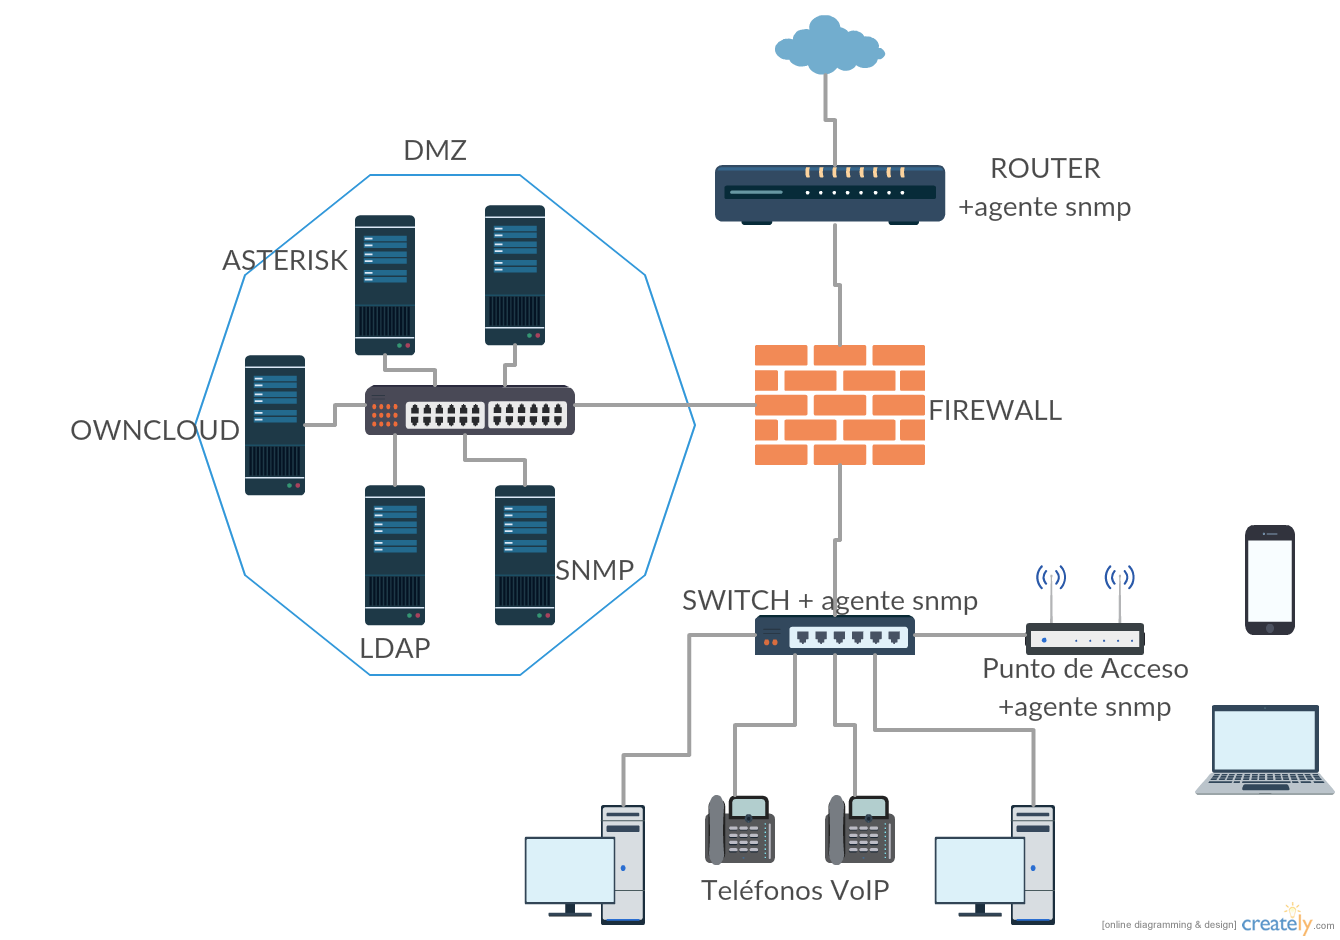
\includegraphics[scale=0.35]{images/topoideal.png}
	\caption{Topología ideal}
	\label{fig:topoideal}
\end{figure}

\subsection{Dispositivos disponibles}

Tenemos para las pruebas y el desarrollo de la práctica, las siguientes herramientas hardware:

\begin{itemize}

	\item Un \textbf{switch} con VLAN y 5 puertos.
	\item Un ordenador que actúa de \textbf{enrutador}, con dos puertos ethernet, uno de ellos con configuración VLAN.
	\item Un \textbf{punto de acceso} WiFi para el acceso a la red.
	\item Un \textbf{iPhone} y un \textbf{portátil Mac}, útiles para probar VOIP con wifi.
	\item Dos ordenadores que actúan como \textbf{organizaciones} 31 y 32.
	\item Dos ordenadores más para simular \textbf{clientes} haciendo peticiones.

\end{itemize}




\subsection{Topología desplegada}

En cuanto a la topología física real, disponemos en el laboratorio de 3 torres, 5 puertos del switch CISCO y un punto de acceso wifi configurado para la organización 31. La conexión de una de las torres como router y las otras dos como equipos de cada organización ya se explica en los boletines de prácticas.

A partir de esa configuración básica, configuramos las dos organizaciones de manera casi simétrica: en la \textbf{máquina física} de cada organización se ejecutarán \textbf{todos los servicios}, es decir, del diseño lógico ideal donde cada servicio tiene una máquina física para él solo, ahora todos los servicios conviven en la misma máquina física. Decidimos usar un servidor físico porque la cantidad de servicios proporcionados por la organización no son tan pesados como \textbf{carga de trabajo} conjunta para una única máquina, como lo pueda ser tener \textbf{varios} servidores como \textbf{máquinas virtuales} en la misma torre del laboratorio.

Ahora bien, por el modo en que programamos la instalación de servicios, nos es muy fácil portarlos desde una máquina física a varias, cambiando las configuraciones de la IP de cada máquina.

En la \autoref{fig:topofisica} vemos el diagrama de la topología física, donde tenemos el ordenador que hace de router, los otros dos ordenadores del laboratorio que actuarán de servidores, el punto de acceso donde usamos nuestros móviles y portátiles personales, y la posibilidad de usar otra torre del laboratorio como cliente.


\begin{figure}[h!]
	\caption{Topología física}
	\centering
		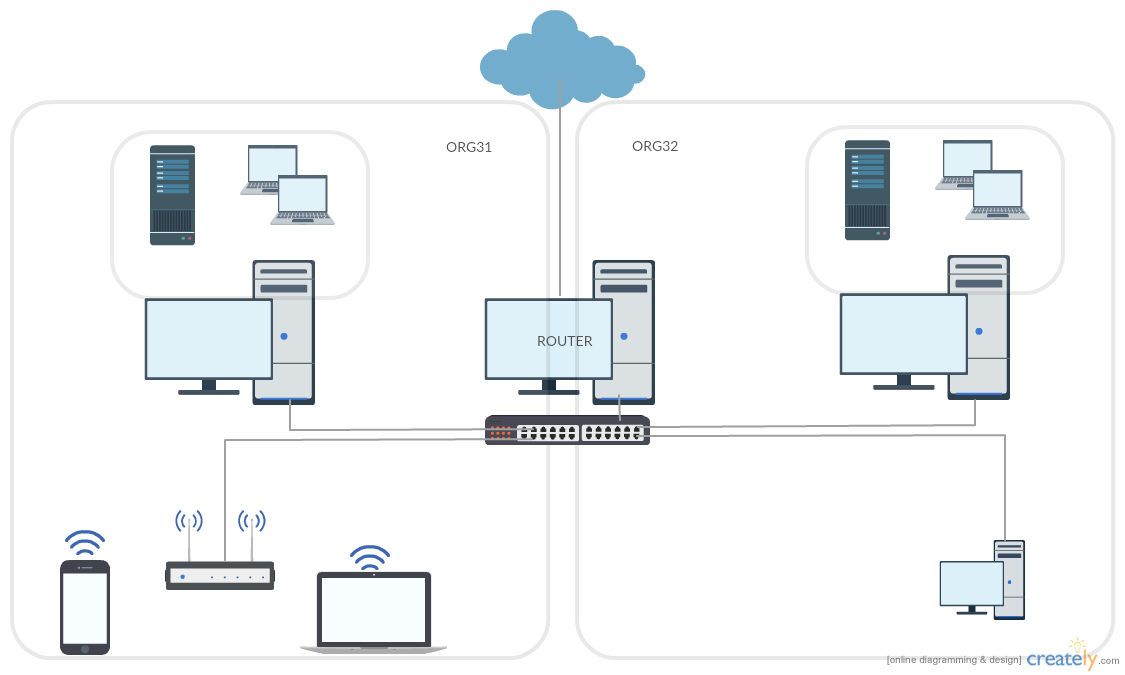
\includegraphics[scale=0.35]{images/TopologiaFisica}
	\label{fig:topofisica}
\end{figure}




\section{Configuración automatizada de los equipos}

Para la configuración de los dispositivos utilizamos herramientas Makefile, y scripts escritos en bash y python, de manera que desplegar los servicios y la topología en un dispositivo esté automatizado, llegando a tal punto que en la instalación sólo haría falta intervenir para escribir la contraseña de la base de datos de Owncloud y pulsar Intro en alguna instalación. No nos apoyamos en una máquina virtual que vayamos configurando a lo largo de las prácticas llevándola de un lado a otro, y por lo general, usamos máquinas virtuales con una instantánea \textit{limpia}.
\\

Usamos una estructura de directorios basada en el hardware a configurar. Es decir, en el ordenador que hace de enrutador ejecutamos un Makefile que está en el directorio ROUTER; para la máquina servidor de la organización 31, la carpeta SERVER correspondiente; etc.

%TODO: decidir si se pone la estructura, y si se modifica cómo presentarla.
\begin{Verbatim}
ROUTER
	SNMP
	Makefile
	network
	test
ORG1
	FISICA
		Makefile
		network
		test
	SERVER
		SNMP
		VOIP
		Makefile
		network
		test
	CLIENTE1
		SNMP
		VOIP
		Makefile
		network
		test

\end{Verbatim}





\section{Servicios}

\subsection{Enrutamiento}

Del enrutamiento se encarga el PC que hace de router. La configuración física se basa en dos puertos Ethernet y VLAN:

\begin{itemize}
	\item Un puerto se usa para conectarse a la red de la UMu, que da conectividad al exterior.
	\item Otro puerto, conectado al \textit{trunk switch vlan} de la organización 31 y 32.
\end{itemize}

La configuración lógica, es decir, la configuración de los interfaces de red es la siguiente:

\lstinputlisting{../ROUTER/network}
%Explicación del fichero: DONE

El script instala el soporte de vlan en el ordenador, desactiva el gestor de redes de ubuntu, copia en \textit{/etc/network/interfaces} la configuración de los puertos ethernet: eth0 conexión a la red UMu con DHCP; eth1.31 y eth1.32 las dos VLAN para el segundo puerto ethernet. A continuación, copia en \textit{/etc/hosts} los nombres correspondientes a las IPs de las máquinas de cada organización, para solventar la falta de un servidor DNS que los registre. Hay máquinas de más de cara a posibles expansiones durante el desarrollo de la práctica. Por último activa el \textit{forwarding} de paquetes y la regla de iptables para actuar como NAT para la subred 192.168.0.0/16, enviando los paquetes por eth0 hacia la red de la UMu.

En las máquinas servidor basta con modificar el fichero \textit{/etc/network/interfaces} para configurar la IP fija 192.168.3i.100 i$ \in \{1,\ 2\} $, pues no tenemos servidor DHCP para autoconfiguración.


\subsection{SNMP}
%Ideal más Intro: DONE

En la topología ideal descrita hemos indicado que habría un servidor dedicado para SNMP. En concreto sería para el manejador, con un acceso por VLAN de gestión desde un ordenador del administrador en la red interna. El resto de servidores, el firewall, el router, los switches y los puntos de acceso inalámbricos tendrían instalados SNMP como agente.

La configuración de cada dispositivo sería:
\begin{itemize}
	\item Todos los dispositivos usarían SNMPv3 y la lectura siempre con autenticación de usuario como mínimo.
	\item El router y firewall, por ser elementos más críticos, además de autenticación, con encriptación, y nunca permisos de escritura.
	\item Los únicos dispositivos con posibilidad de escritura serían los switches y puntos de acceso en la red interna, y añadiendo encriptación.
	\item Los traps (quitando el caso de que no funcionara \textit{monitor}) serían:
		\subitem En los switches, cuando la interfaz donde se conecta un punto de acceso u otro switch esté caída.
		\subitem En los servidores, cuando la interfaz o puerto del servicio que dan, más los básicos como SSH, estén caídos. El trap de la interfaz sólo llegaría si tuviera más de una conectada a la subred.
		\subsubitem En el servicio Owncloud y VoIP cuando el ancho de banda llegue al 80\% de la capacidad máxima, por ser servicios que dependen de buena conexión para una correcta experiencia de uso.
		\subsubitem En Owncloud además, si el espacio de disco duro libre es inferior al 30\%.
\end{itemize}

\hfill

En nuestra topología de prácticas, cada organización tiene un manejador en la máquina física, y como agentes la propia máquina y el router, que al ser también la misma máquina para ambos, en su configuración como agente incluye los \textit{community} de ambas organizaciones.

En cuanto a la seguridad, el router tendrá sólo acceso de lectura con autenticación y cifrado de los mensajes; el servidor de la organización también tendrá permisos de sólo lectura, pero el acceso se relaja a autenticación sin cifrado.

Por problemas descubiertos con los paquetes de SNMP donde la orden \textit{monitor} no funciona, con posible solución la compilación de los paquetes snmp, decidimos instalar en el servidor de la organización 31 Nagios, añadiendo la monitorización de disco y ancho de banda del router, como se explicará en su sección.

\subsubsection{Agentes}
%TODO
\subsubsection{Manejador}
%TODO

\begin{Verbatim}[frame=single]

$snmpwalk -v 3 -c sta31 -u router -l authPriv -a MD5 -A 123456789
 -x DES -X 123456789 192.168.31.1 1.3.6.1.2.1.2.2.1.2

IF-MIB::ifDescr.1 = STRING: lo
IF-MIB::ifDescr.2 = STRING: eth1
IF-MIB::ifDescr.3 = STRING: eth0
IF-MIB::ifDescr.4 = STRING: eth1.31
IF-MIB::ifDescr.5 = STRING: eth1.32

$snmpwalk -v 3 -c sta31 -u router -l authNoPriv -a MD5 -A 123456789 
192.168.31.1 1.3.6.1.2.1.2.2.1.2

IF-MIB::ifDescr.1 = STRING: lo
IF-MIB::ifDescr.2 = STRING: eth1
IF-MIB::ifDescr.3 = STRING: eth0
IF-MIB::ifDescr.4 = STRING: eth1.31
IF-MIB::ifDescr.5 = STRING: eth1.32
\end{Verbatim}


\subsubsection{Nagios}
%TODO

\begin{center}
	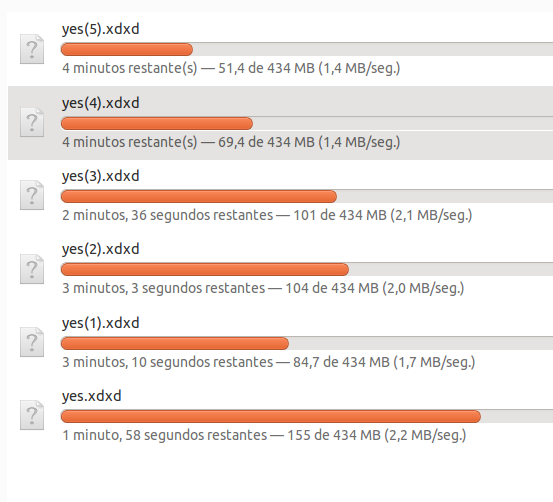
\includegraphics[scale=0.5]{images/snmp/nagios/descargas.png}
\end{center}
\begin{center}
	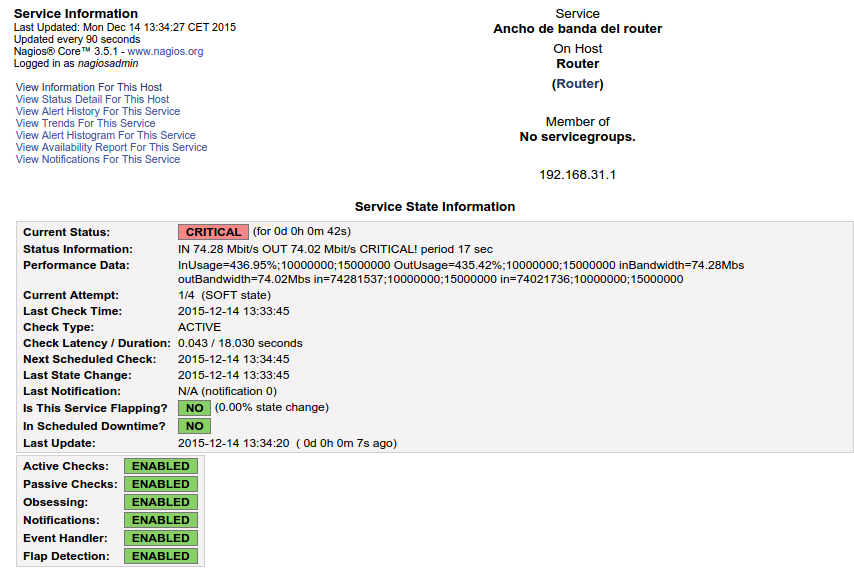
\includegraphics[scale=0.5]{images/snmp/nagios/critical bandwidth.png}
\end{center}

\subsection{Voz sobre IP}
%TODO
En esta sección documentamos las configuraciones que hemos tomado para el servidor de Asterisk.

\subsubsection{Configuración básica}
%TODO
Para las organizaciones 31 y 32, hacemos 2 cuentas de cliente para ambas organizaciones (311 y 312 para organización 31; 321 y 322 para la organización 32).

\begin{lstlisting}
TODO: Copiar aqui la configuracion relativa a los clientes.
\end{lstlisting}

Para esos clientes también hemos configurado sus extensiones.

\begin{lstlisting}
TODO: Copiar aqui la configuracion relativa a las extensiones.
\end{lstlisting}

\subsubsection{Troncales Asterisk}
%TODO
Para empezar, hacemos una redirección básica entre los dos servicios Asterisk en las configuraciones de extensión de Asterisk:
\begin{lstlisting}
TODO: Copiar aqui la configuracion relativa a las extensiones entre servicios.
\end{lstlisting}


\subsubsection{Seguridad IPsec}
%DONE

Para proteger la comunicación entre las centralitas de las organizaciones 31 y 32 aplicamos protección por IPsec entre las direcciones de las centralitas, gracias a que elegimos \textit{directmedia=no}, sabemos que cualquier comunicación externa pasará por la centralita y estará protegida. Como en la configuración de la centralita sólo permitimos llamadas en la organización y sólo sabemos redirigir a la organización 31 o 32, también sabemos que no habrá llamadas externas sin proteger.

Sin embargo, en la topología ideal, la aplicación de IPsec se haría en las comunicaciones entre los routers, protegiendo así no sólo el servicio VoIP, sino todas las comunicaciones entre las organizaciones. Como sólo tenemos un router, en la práctica IPsec se instala entre cada servidor de las organizaciones, y para poder analizar los mensajes, no usamos ESP, sólo AH.

Además, en la solución ideal, en caso de que aceptemos llamadas entre otras organizaciones además de la 31 y 32, añadiríamos seguridad TLS o DTLS para UDP, entre la centralita y el otro extremo. En nuestra práctica con IPsec es más que suficiente, y al tener todos los servicios en la misma máquina, todos se benefician como si fuera IPsec entre los routers.

\hfill

La instalación de IPsec se puede seguir en las diapositivas de Servicios Telemáticos del año pasado. Basta con modificar \textit{/etc/ipsec-tools.conf} en ambas máquinas añadiendo para AH, en la máquina de la organización 31:

\begin{Verbatim}[frame=single]
add 192.168.31.100 192.168.32.100 ah 0x200 -A hmac-md5 0xc0291ff014dccdd03874d9e8e4cdf3e6;
add 192.168.32.100 192.168.31.100 ah 0x300 -A hmac-md5 0x96358c90783bbfa3d7b196ceabe0536b;

spdadd 192.168.31.100 192.168.32.100 any -P out ipsec ah/transport//require;
spdadd 192.168.32.100 192.168.31.100 any -P in ipsec ah/transport//require;
\end{Verbatim}


O en caso de poner ESP, en la organización 31:

\begin{Verbatim}[frame=single]
add 192.168.31.100 192.168.32.100 esp 0x201 -E 3des-cbc
 0x7aeaca3f87d060a12f4a4487d5a5c3355920fae69a96c831 -A hmac-md5 0xc0291ff014dccdd03874d9e8e4cdf3e6;
add 192.168.32.100 192.168.31.100 esp 0x301 -E 3des-cbc
 0xf6ddb555acfd9d77b03ea3843f2653255afe8eb5573965df -A hmac-md5 0x96358c90783bbfa3d7b196ceabe0536b;

spdadd 192.168.31.100 192.168.32.100 any -P out ipsec esp/transport//require;
spdadd 192.168.32.100 192.168.31.100 any -P in ipsec esp/transport//require;
\end{Verbatim}

Para la organización 32 es igual cambiando los out por in, y viceversa.

\hfill
\\


Y con un simple ping desde una máquina a la otra podemos ver cómo se añaden las cabeceras AH a los paquetes, en la \autoref{fig:pingreqAH} vemos el ping request y que el campo AH SPI corresponde al 0x200 de la configuración, y en la \autoref{fig:pingreplyAH} del ping reply, el valor es el 0x300 de las comunicaciones desde 192.168.32.100 a 192.168.31.100.


\begin{figure}[h!]
	\caption{Ping Request AH}
	\centering
	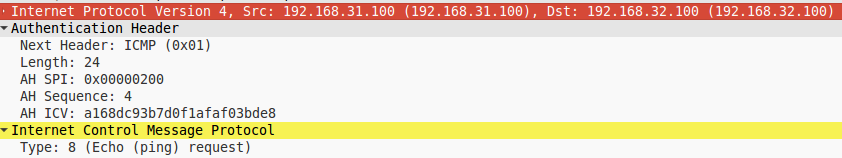
\includegraphics[scale=0.5]{images/ipsec/pingreqAH.png}
	\label{fig:pingreqAH}
\end{figure}

\begin{figure}[h!]
	\caption{Ping Reply AH}
	\centering
	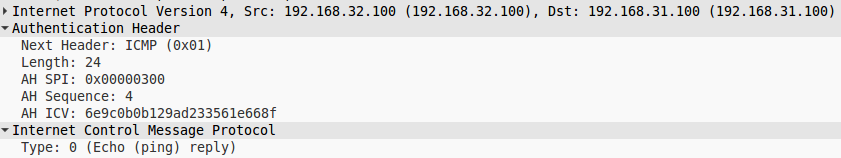
\includegraphics[scale=0.5]{images/ipsec/pingreplyAH.png}
	\label{fig:pingreplyAH}
\end{figure}



\subsubsection{Buzón de voz}
%TODO





\subsection{LDAP}
El servicio LDAP ofrece al resto de servicios un punto en común donde encontrar la información relevante de los usuarios (nombres,
organización a la que pertenecen, permisos de uso y acceso, credenciales, etc).

Como contiene la información crítica de los usuarios que se integran en los servicios, LDAP se despliega en su propia máquina.

Sin embargo, en el despliegue real del laboratorio, LDAP está integrado en el ordenador de la organización 31.

Para las pruebas de laboratorio, la instalación y la configuración la generamos automáticamente (sin necesidad de interacción del administrador), en python, generando tres clientes de la organización 31.

Estos tres clientes se generan con el servicio Owncloud en mente. Para organizar la pertenencia de usuarios de Owncloud en el árbol, hemos decidido usar el campo Organizational Unit con valor \textit{owncloud} para indicar la pertenencia al servicio.
                                                                                                                                                                                                                                                                     
Este caso es el más sencillo para aplicar en nuestro caso práctico, pero no es el mejor para la topología ideal. El servicio ldap no lo suele usar un único servicio, y no todos los usuarios tienen acceso a los mismos servicios en una organización. Por ejemplo, el servicio Golum de la Universidad de Murcia frente al de correo o UmuBox.

La solución ideal sería tener los usuarios registrados sin indicar los servicios por la \textit{ou}, sino crear un grupo por cada servicio, y del que cuelguen identificadores de los usuarios que pertenecen al grupo. Así, un usuario registrado en ldap tiene una sola entrada con todos sus datos, y cuelga de una sola \textit{ou}, no de varias posibles, y para asignarle a un servicio, sólo hay que ir al nodo del servicio y dar de alta la hoja del usuario.

Ejemplo de entrada ldap: \textit{cliente311.ldif}:

\begin{BVerbatim}
# Entrada para los usuarios:
dn: cn=cliente311, ou=owncloud, dc=org31, dc=es
changetype: add
objectclass: inetOrgPerson
sn:Perez
cn: cliente311cn
uid: cliente311uid
userPassword: manyhue
ou:owncloud
\end{BVerbatim}

%TODO: Indicar puertos usados.
%TODO: hacer consulta entre organizaciones, con un ldapsearch más simple

A continuación se muestran imágenes de la traza capturada durante la orden: \textit{ldapsearch -x -b “dc=org11,dc=es"\ “ou=owncloud"\ dn description}:

Las dos primeras trazas indican el acceso a ldap. Las dos últimas indican que la búsqueda ha terminado con éxito y que se puede terminar la consulta.

\begin{center}
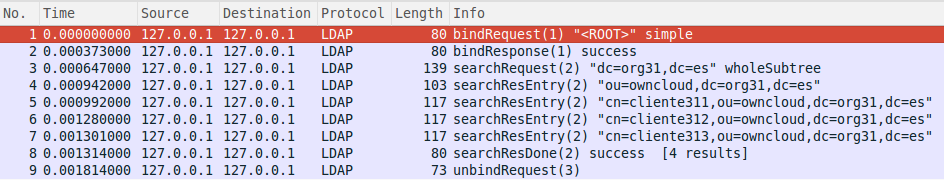
\includegraphics[scale=0.5]{images/ldap/ldap1}
\end{center}

Aquí se muestra la tercera traza con la petición de búsqueda del comando, con el objeto \textit{“dc=org11,dc=es"} como punto inicial de búsqueda, el filtro de \textit{“ou=owncloud"} y los atributos a devolver \textit{dn} y \textit{description}.

\begin{center}
	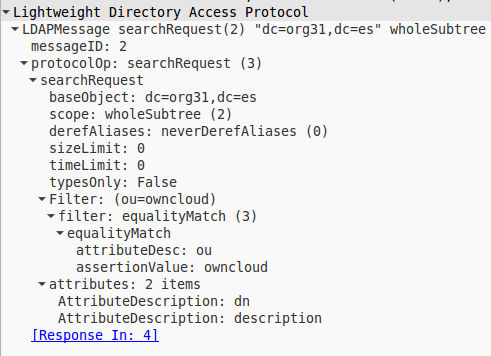
\includegraphics[scale=0.5]{images/ldap/ldap2}
\end{center}

Las siguientes imágenes muestran los resultados (\textit{searchResEntry}), con la entrada que define la propia O.U. Owncloud, seguido de las entradas de los clientes \textit{cliente311}, \textit{cliente312} y \textit{cliente313}.

\begin{center}
	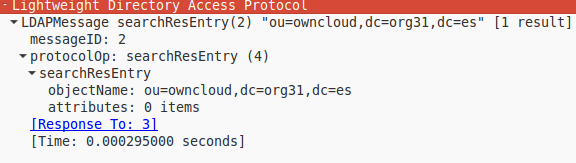
\includegraphics[scale=0.5]{images/ldap/ldap3}
\end{center}
\begin{center}
	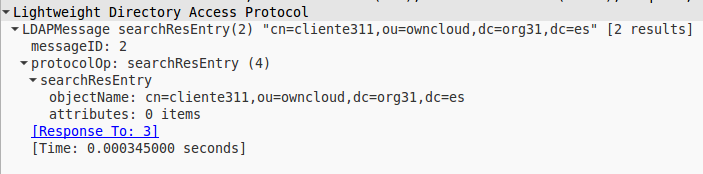
\includegraphics[scale=0.5]{images/ldap/ldap4}
\end{center}
\begin{center}
	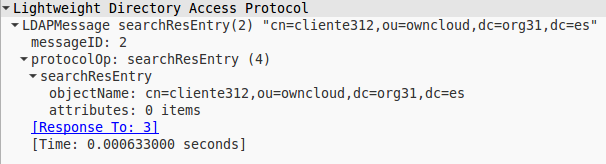
\includegraphics[scale=0.5]{images/ldap/ldap5}
\end{center}

\begin{center}
	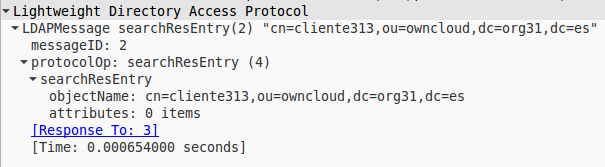
\includegraphics[scale=0.5]{images/ldap/ldap6}
\end{center}




\subsection{OwnCloud}
%TODO
\section{Políticas de seguridad}
%TODO: Un dibujo del escenario de seguridad

\subsection{Análisis de riesgos}
%TODO: Tabla de reglas de seguridad
El escenario tiene como servicios a proteger:

\begin{itemize}
	\item LDAP
	\item OwnCloud
	\item Voz sobre ip
	\item SNMP + Nagios3
\end{itemize}

De estos servicios los únicos que tienen que ofrecer funcionalidad al exterior son OwnCloud (que está localizado en la organización 31) y VOIP (con dos servidores dedicados ASTERIX, uno en cada organización).

Por lo tanto, los otros dos servicios (SNMP y LDAP) hay que protegerlos completamente de accesos al exterior. 

Como LDAP es un servicio crítico (contiene el directorio de usuarios, y se usa para otros servicios), en un escenario real LDAP estaría en su propia máquina con todo capado salvo el acceso desde el servidor OwnCloud que necesita acceso para los usuarios registrados.

La máquina con Nagios3 haría de centro de control. Sería la única con acceso ssh al exterior y la única desde la cual se puede hacer ssh al resto de servidores (y al router), además de monitorizar todos los dispositivos con Nagios y SNMP.

En este escenario, para poder manipular remotamente el servicio LDAP por ejemplo se necesitaría acceder al servidor de Nagios y después al de LDAP, duplicando la seguridad. En caso de que el servidor de Nagios estuviera comprometido, todavía haría falta un nivel más de acceso para poder llegar al LDAP.




\subsection{Configuración de seguridad}
%TODO: Iptables

\subsection{Generación de certificados}

La creación de una jerarquía de certificados con su CA no se establece como un servicio a desplegar para el público o clientes, pero lo necesitamos en esta práctica de cara a la seguridad TLS de Owncloud.

En el caso ideal de nuestra organización, de ofrecer el servicio de nuestra CA para firmar solicitudes de certificados dispondríamos una máquina física en la red DMZ cuya única función sea la de almacenar la clave privada de la CA, firmar las solicitudes y por supuesto generar las lístas de CRL publicándolas en el servidor web. Esta máquina es tan crítica en la seguridad que dispondría de un firewall que la aislara del tráfico de la red DMZ como una segunda capa de seguridad, donde sólo se permitan comunicaciones desde el servidor para el intercambio de ficheros criptográficos, y el servidor HTTP/S donde registrarse por primera vez.

Siguiendo el ejemplo de otras CA, el procedimiento para firmar un certificado de un servidor web sería: el cliente registra el dominio que quiere que se certifique, se le indica que instale un script en el servidor, el cual escuchará las conexiones proactivas del servidor de la CA, que hará una comprobación con datos aleatorios para comprobar que es la máquina del dominio indicado y el script instalado, se le indica al script que genere el par de claves y el csr, se envía responde a la CA con el csr y ésta termina devolviendo el certificado público firmado. De esta manera, la única comunicación que recibiría la CA sería la dirección del servidor, y el resto de comunicaciones las iniciaría la máquina de la CA. Es más, el servidor web sería el que dispusiera el formulario de registro y la única máquina que el nuevo firewall permitiera comunicarse con el servidor de la CA.

Para administración, el firewall añadiría un acceso por ssh desde una máquina específica de un administrador del sistema desde la red interna a la organización, y por una VLAN reservada exclusivamente para dicho propósito.

Teniendo en cuenta que tratamos con la clave privada de nuestra CA, nunca se es demasiado paranoico.


\hfill


En nuestro caso práctico, las claves de la CA para generar los CRL se encuentra en la misma máquina que el resto de servicios (nada recomendable), y para generar las claves seguimos los pasos de las diapositivas de prácticas, añadiendo los siguientes detalles:

\begin{itemize}
	\item En el fichero \textit{openssl.conf} en la sección $[$ usr\_cert $]$, la que indica qué hay que hacer al firmar una solicitud csr, hay que añadir la línea \textit{crlDistributionPoints = URI:http://server.org31/crl/org31.CRL} para indicar, en los certificados firmados, que la CA generará las listas de CRL y las publicará en la dirección \textit{http://server.org31/crl/org31.CRL}, que en nuestro caso es el mismo servidor apache2 que Owncloud.
	\item El certificado del servidor hay que darle como \textit{common name} \textit{server.org31}, que es el nombre por el que accederemos desde el navegador, el escrito en \textit{/etc/hosts} a falta de servidor DNS.
	\item Con crontab añadimos el comando de generar una nueva lista actualizada de los CRL a las doce de la noche cada día, copiándola en el servidor web indicado antes.
	\item Al servidor apache2, en la configuración de SSL se le debe indicar dónde está su certificado, que compruebe el certificado de los clientes y haga una comprobación de los certificados revocados por la lista CRL.
	\subitem Para la comprobación de CRL se debe indicar un fichero (o una carpeta con ficheros nombrados por hash) donde se encuentre un fichero CRL correcto.
	\subitem Entre los problemas que nos hemos ido encontrando en el despliegue, se encuentra que Apache no comprueba la lista de CRL indicada con la extensión del primer punto, sino que siempre compara con el fichero indicado, y en caso de modificar el fichero, se debe reiniciar el servicio. Por ello, para las pruebas de revocación, se copia `forzosamente' el CRL actualizado en el fichero de Apache, aunque se siga publicando en la dirección web.
\end{itemize}

\hfill

Para las pruebas, tenemos el certificado de la CA, el de \textit{server.org31} y el de \textit{cliente}, no necesitamos más en las pruebas, pues sólo tenemos un servidor y el certificado de cliente es para comprobar la revocación, no hemos añadido que sirva para iniciar sesión en Owncloud en vez de escribir usuario y contraseña.

Primero comprobamos que sin el certificado el servidor no nos deja acceder a Owncloud por HTTPS en la \autoref{fig:pedircert}, después, que con el certificado del cliente, \autoref{fig:usercert1} y \autoref{fig:usercert2}, sin revocar nos permite acceder,  \autoref{fig:https}, y finalmente revocamos el certificado de \textit{cliente}, actualizamos el CRL, lo copiamos en el fichero de Apache, reiniciamos el servidor, y volvemos a intentar acceder, recibiendo un error por la revocación del certificado, en \autoref{fig:revoked}.

%TODO: imagenes de las pruebas de los certificados de servidor, cliente y revocación

\begin{figure}[h]
	\caption{Petición certificado de cliente}
	\centering
	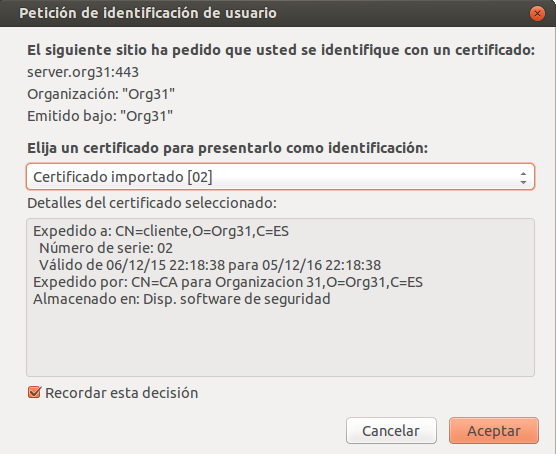
\includegraphics[scale=0.5]{images/certs/pedircert.png}
	\label{fig:pedircert}
\end{figure}


\begin{figure}[h]
	\caption{Conexión HTTPS}
	\centering
	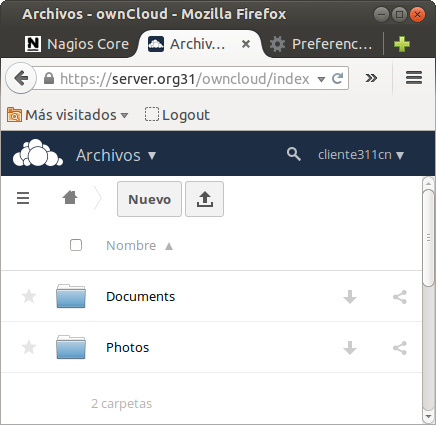
\includegraphics[scale=0.5]{images/certs/https.png}
	\label{fig:https}
\end{figure}

\begin{figure}[h]
	\caption{Certificado de usuario 1/2}
	\centering
	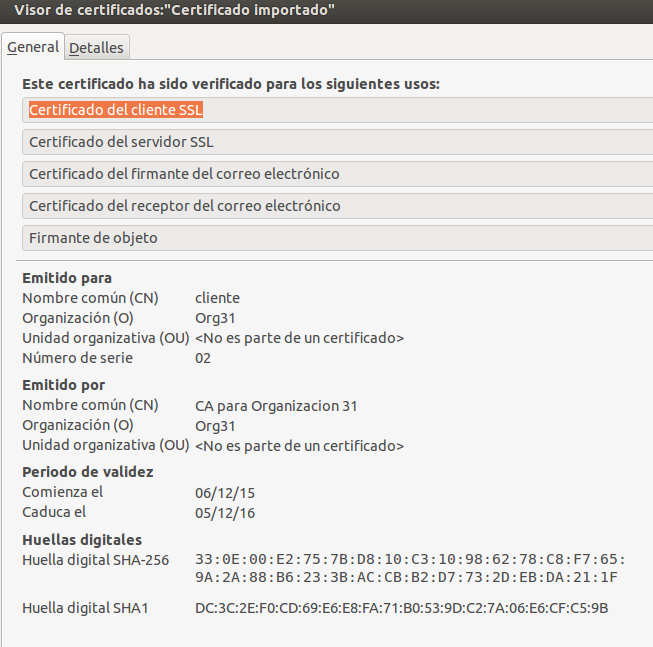
\includegraphics[scale=0.5]{images/certs/usercert1.png}
	\label{fig:usercert1}
\end{figure}


\begin{figure}[h]
	\caption{Certificado de usuario 2/2}
	\centering
	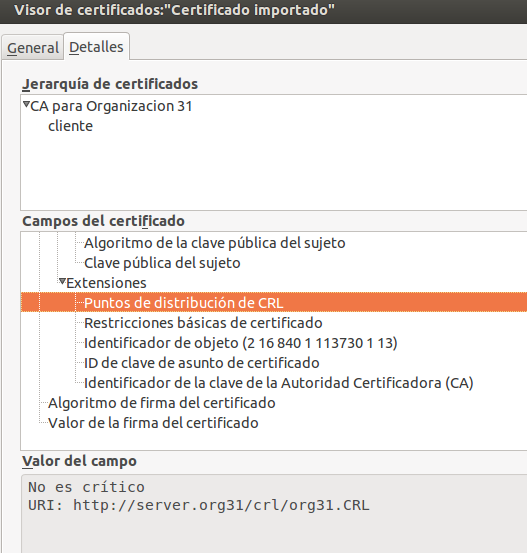
\includegraphics[scale=0.5]{images/certs/usercert2.png}
	\label{fig:usercert2}
\end{figure}

\begin{figure}[h]
	\caption{Certificado del servidor}
	\centering
	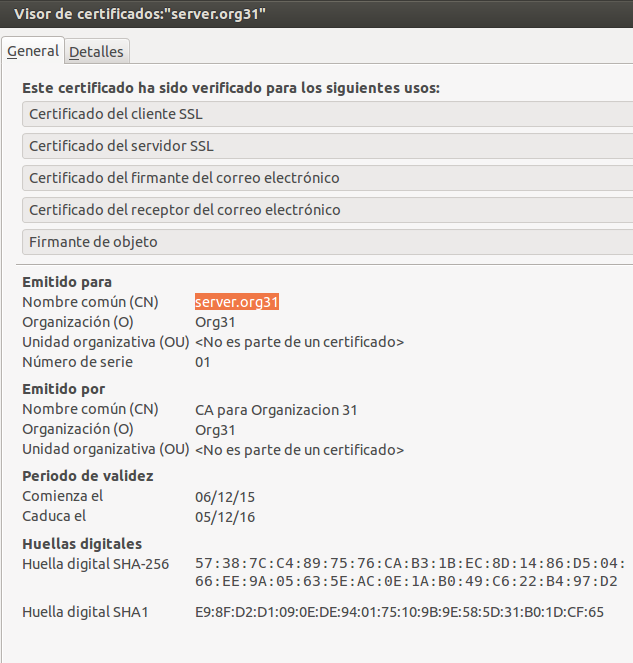
\includegraphics[scale=0.5]{images/certs/servercert1.png}
	\label{fig:servercert1}
\end{figure}

\begin{figure}[h]
	Revocación del certificado de \textit{cliente}:
\begin{Verbatim}[frame=single]
alumno@Laboratorio27:~/demoCA$ openssl crl -in /var/www/crl/org31.CRL -text -noout 
	Certificate Revocation List (CRL):
		Version 2 (0x1)
	Signature Algorithm: sha256WithRSAEncryption
		Issuer: /C=ES/O=Org31/CN=CA para Organizacion 31
		Last Update: Dec 14 18:29:43 2015 GMT
		Next Update: Jan 13 18:29:43 2016 GMT
		CRL extensions:
			X509v3 CRL Number: 
				2
	Revoked Certificates:
		Serial Number: 02
	Revocation Date: Dec 14 18:28:56 2015 GMT
	Signature Algorithm: sha256WithRSAEncryption
		a7:a6:7d:75:92:81:4f:e1:21:b4:db:58:5b:60:dd:b8:12:0c:
		9f:83:53:d0:41:59:34:2c:d1:e4:d2:56:a9:ce:01:b5:8e:4f:
		53:0f:f4:40:1c:95:d6:55:77:9f:82:a2:d1:fc:b4:07:dd:46:
		d0:bd:d3:47:c3:46:7a:cb:af:e6:09:86:55:68:eb:dd:f2:8b:
		19:a0:91:d5:5c:d2:e7:1e:7f:38:a1:31:de:6a:2e:e6:cb:d5:
		fa:af:02:33:12:34:47:22:8a:41:da:ff:96:bb:ca:52:72:b9:
		11:97:e7:20:46:44:e5:13:5d:9d:5a:da:34:71:d4:09:87:f4:
		7a:2d:d5:6c:d6:ea:b0:6b:4e:db:28:f4:c9:81:ef:b1:16:43:
		50:b7:be:9e:e6:95:af:60:ce:8f:ad:9c:99:f3:f7:2e:24:5a:
		92:13:03:b4:a8:d8:e9:e2:05:b7:89:95:d0:07:88:d4:d8:99:
		bd:5f:2c:35:8c:18:90:d9:d3:93:80:db:ea:4f:e6:83:d1:7c:
		b2:83:ce:fb:c5:6b:3c:15:af:bb:31:1b:42:7e:44:44:b5:d8:
		a3:ca:fd:0e:0c:ac:ab:b5:b0:47:8e:00:65:cd:e1:d0:e2:5b:
		5d:55:5e:d8:43:96:8d:cc:55:6c:ee:a0:3b:c0:bb:b7:80:bc:
		3c:ec:30:c2
\end{Verbatim}
\end{figure}


\begin{figure}[h]
	\caption{Certificado de cliente revocado}
	\centering
	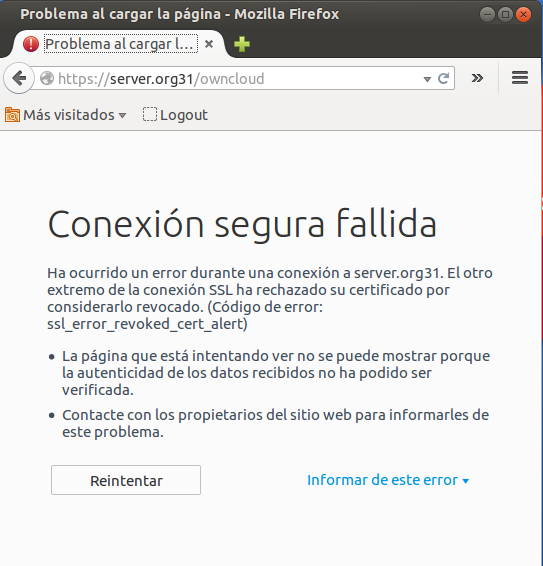
\includegraphics[scale=0.5]{images/certs/revoked.png}
	\label{fig:revoked}
\end{figure}




               
   

\end{document}
\grid
